% ----------------------------------------------------------------------- %
% Arquivo: cap3.tex
% ----------------------------------------------------------------------- %
\chapter{\Large{\textbf{Arquitetura dos Dispositivos Móveis}}}
\label{c_cap3}


Nesse  capítulo será abordado o  histórico da evolução dos dispositivos móveis e apresentará os Sistemas Operacionais mais famosos que são o IOS e Android, de modo a traçar um paralelo entre eles.

\section{Evolução dos Dispositivos Móveis}
Atualmente, os dispositivos móveis, são imprescindíveis na vida das pessoas. Quem imaginaria que no começo eles que tinham recursos muito limitados, poucas funcionalidades, se restringindo basicamente a serem calculadoras, e hoje, tem-se praticamente computadores pessoais em nossas mãos, tanto, em relação a funcionalidades quanto na questão de poder de processamento. A medida que, os dispositivos móveis foram evoluindo, novas funcionalidades foram aparecendo, calendário, rádio, jogos, mas foi quando a Apple lançou seu primeiro smartphone, o Iphone, com seu próprio \ac{SO} o IOS, e a Google lançou o seu \ac{SO} para smartphones, o Android, que os dispositivos móveis ganhariam a fama de hoje. Com esses sistemas abriu se um leque de oportunidades para empresas e programadores avulsos, à desenvolverem os mais diversos aplicativos.

O marco da telefonia móvel se deu no ano de 1973, quando dois engenheiros da Motorola, realizaram a primeira ligação da história feita a partir de um telefone móvel, o modelo era o então, DynaTAC como mostra a \autoref{motorola}. Com seus poucos mais  de 30 cm de tamanho e peso de quase 1kg, o seu lançamento só ocorreu no ano de 1983, 10 anos após a demonstração \cite{historia_mobile}.

\begin{figure}[!htpb]
	\centering
	\caption{Motorola DynaTAC}
	\frame{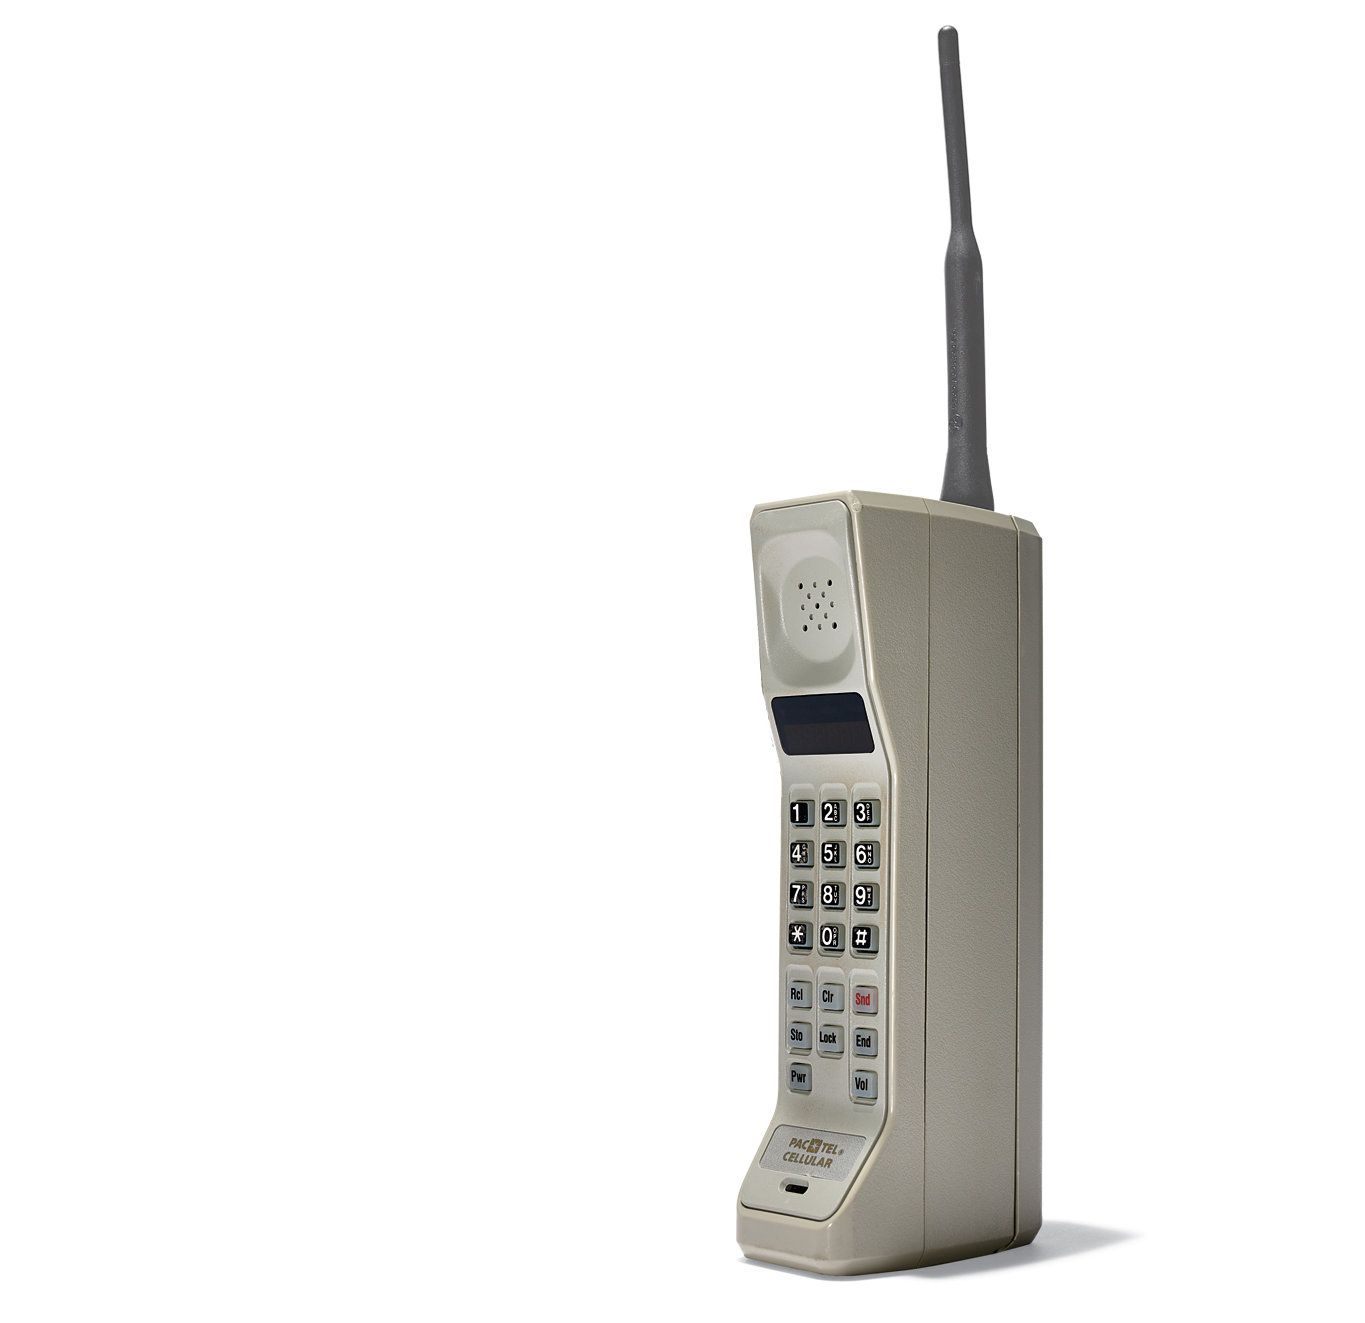
\includegraphics[scale=0.20]{images/motorola_dynatac.jpg}}\\
	{\footnotesize Fonte: \cite{motorola_dynatac}}
	\label{motorola}
\end{figure}

A primeira geração de telefones móveis, teriam as mesmas características do DynaTAC, não sendo tão portáteis, mas era o primeiro passo e a tendência seria que esses aparelhos evoluíssem e aumentasse suas funcionalidades \cite{historia_mobile2}.

No ano de 1994, a IBM lança o Simon, um aparelho que reunia diversas funcionalidades, dentre elas \ac{PDA} e Fax, e foi um grande passo para o desenvolvimento dos dispositivos móveis, sendo o precursor da tela \textit{touchscreen}, mas suas medidas ainda eram muito grandes e acabou não sendo tão popular, vendendo apenas 50 mil unidades \cite{historia_mobile}.  A \autoref{simon}
mostra o Simon.

\begin{figure}[!htpb]
	\centering
	\caption{IBM Simon}
	\frame{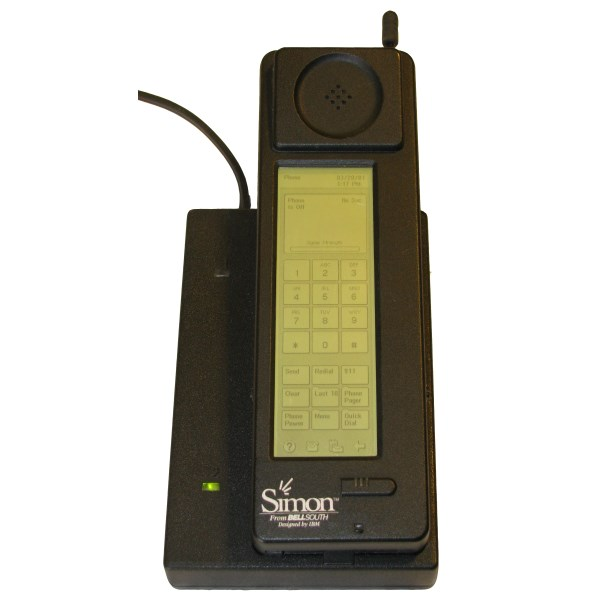
\includegraphics[scale=0.30]{images/IBM_Simon.jpg}}\\
	{\footnotesize Fonte: \cite{historia_mobile}}
	\label{simon}
\end{figure}

Na \autoref{nokia9} é possível ver o Nokia Communicator 9000 que foi um aparelho que fez bastante sucesso, lançado em 1996, foi o primeiro dispositivo móvel comercializado com acesso a internet, além disso reunia diversas funcionalidades como,  FAX, SMS, e-mail, agenda de contatos, calculadora, bloco de anotações e outras mais. Suas medidas ainda eram grandes, mas possuía um o recurso de flip, em que tinha uma segunda tela e um teclado QWERTY \cite{historia_mobile}.

\begin{figure}[!htpb]
	\centering
	\caption{Nokia 9000}
	\frame{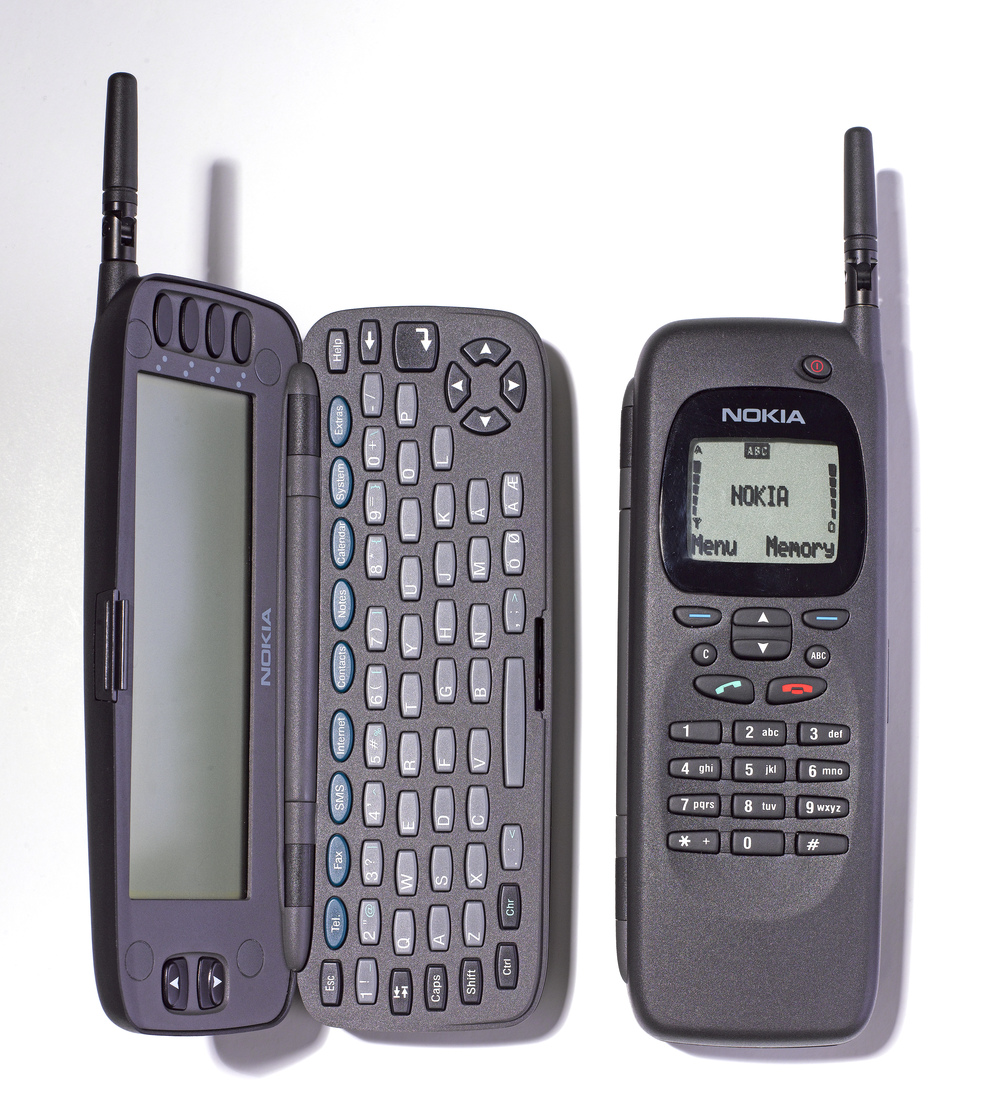
\includegraphics[scale=0.8]{images/nokia_communicator_9000.jpg}}\\
	{\footnotesize Fonte: \cite{nokia_9000}}
	\label{nokia9}
\end{figure}

\newpage
Em janeiro de 2007, Steve Jobs em uma apresentação da Apple, lança um smartphone que mudaria tudo, o IPhone. Com design minimalista, o IPhone dispensou o uso de teclas físicas, tudo seria a base do toque na tela como mostra a \autoref{apple} \cite{historia_mobile2}.

\begin{figure}[!htpb]
	\centering
	\caption{Primeiro IPhone}
	\frame{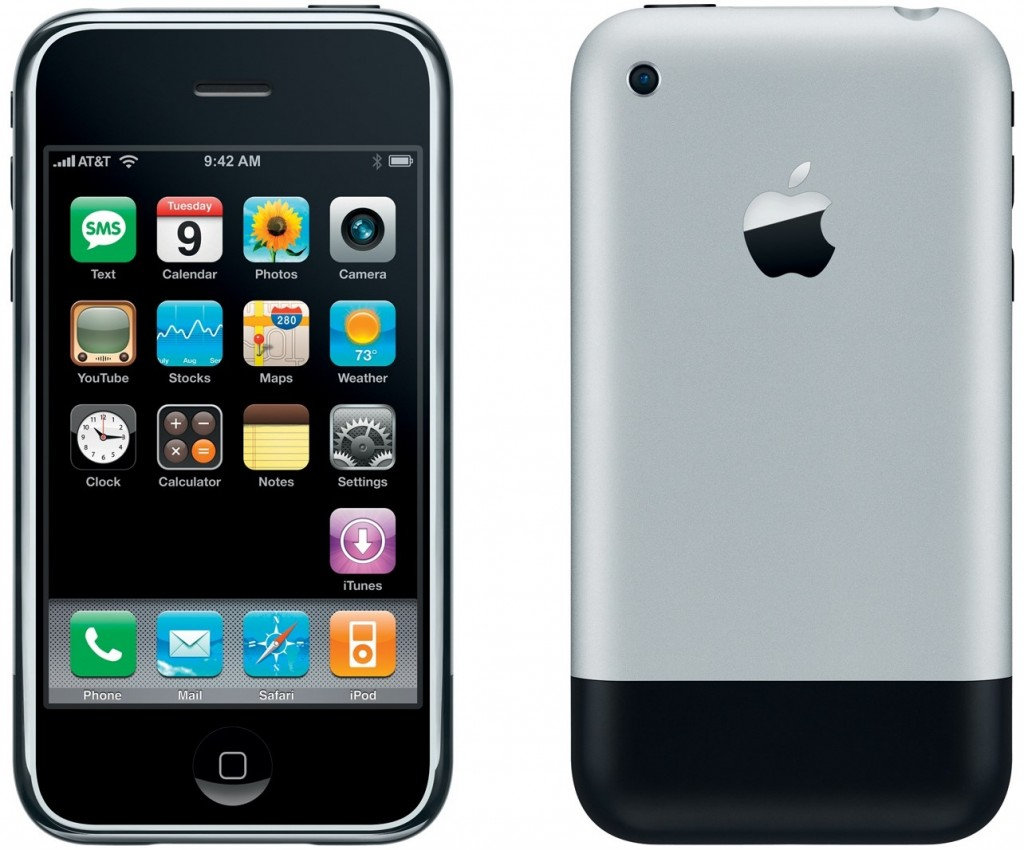
\includegraphics[scale=0.22]{images/iPhone.jpg}}\\
	{\footnotesize Fonte: \cite{historia_mobile}}
	\label{apple}
\end{figure}

A Apple desenvolveu um \ac{SO} próprio para o dispositivo, o IOS, um sistema operacional de fácil interação para o usuário que o tornou bastante popular. Além disso, com o  IPhone surgiram também os aplicativos, inicialmente vindos apenas de fábrica, e depois comprados pela loja virtual, a App Store \cite{historia_mobile}.

Em 2008 surgiria um novo \ac{SO} que entraria na concorrência com o IOS da Apple, o smartphone T-Mobile G1, era lançado com um \ac{SO} desenvolvido pela Google, o Android, ele também trazia uma loja de aplicativos, a Android Market que depois passou a ser chamada como é hoje, Google Play. Com o tempo o Android ganhou espaço e hoje a maioria dos smartphones usam o \ac{SO} da Google \cite{historia_android}.

\section{iOS}
Segundo \cite{ios} "O iOS é um sistema operacional desenvolvido pela Apple que pode ser encontrado no iPhone, iPad e iPod Touch da empresa, visto que os notebooks da empresa utilizando o MacOS e os relógios inteligentes o watchOS."

\section{Android}
De acordo com \cite{android} "Android é o sistema operacional móvel do Google. Presente em múltiplos aparelhos de diversas fabricantes, como Samsung, Motorola, LG, e Sony, é a plataforma mobile mais popular do mundo. É conhecido por ser baseado no núcleo do Linux, ter um código aberto e uma série de possibilidades de personalização."
\label{s_c3_historia}